\documentclass[11pt]{article}
\usepackage{booktabs,natbib,graphicx}


\begin{document}
	
\section*{Draft table for additional benchmarks}
	

\begin{table}[htbp]	
\centering
\begin{tabular}{lcccc}
& Fall,&  Spring,  & 
Fall, & Spring, \\ 
& Current & Current & Next & Next \\ \toprule
IMF & & & & \\ \midrule
AR(1) & & & & \\	
AR(1) -- direct & & & & \\	
AR($p$) & & & & \\	
AR($p$) -- direct & & & & \\	
SV-BVAR & & & & \\	
SV-BVAR -- direct & & & & \\	
SV-BVAR -- direct+CISS & & & & \\	
BVAR & & & & \\	
BVAR -- direct & & & & \\	
BVAR -- direct+CISS & & & & \\\bottomrule
\end{tabular}
\caption{Inflation: Average interval scores over all countries.}
\end{table}

\begin{table}[htbp]	
	\centering
	\begin{tabular}{lcccc}
		& Fall,&  Spring,  & 
		Fall, & Spring, \\ 
		& Current & Current & Next & Next \\ \toprule
		IMF & & & & \\ \midrule
		AR(1) & & & & \\	
		AR(1) -- direct & & & & \\	
		AR($p$) & & & & \\	
		AR($p$) -- direct & & & & \\	
		SV-BVAR & & & & \\	
		SV-BVAR -- direct & & & & \\	
		SV-BVAR -- direct+CISS & & & & \\	
		BVAR & & & & \\	
		BVAR -- direct & & & & \\	
		BVAR -- direct+CISS & & & & \\\bottomrule
	\end{tabular}
	\caption{GDP growth: Average interval scores over all countries.}
\end{table}

\begin{itemize}
	\item If we include CISS here, we might drop Figure 10 from paper. 
	\item Does BVAR-CISS in Figure 10 refer to the direct or standard version of BVAR? In the former case, it should be called BVAR-direct+CISS 
\end{itemize}

\section*{Text snippets}

In the main paper, we consider an AR(1) benchmark model, with forecast distributions constructed based on past forecast errors as for the IMF method. Here we consider additional variants of the AR model. 

First, we consider choosing the AR lag length $p$ based on the \cite{Schwarz1978} information criterion as stated in Equation 4.3.9 of \cite{Luetkepohl2005} and discussed in Section 4.3 of the latter reference. Figure \ref{fig:lag_length_choice} provides an overview of the lag orders chosen in the empirical analysis. While we allowed for a maximal lag order of eight, the largest order chosen in practice was six. For inflation, lag orders between three and five are most common, whereas choices for GDP are clearly smaller, with one being the most popular and three being the maximal choice. 

Second, we consider using the analytical forecast distribution implied by the AR model, as opposed to the empirical distribution of its past forecast errors. We call this approach AR--direct, in analogy to our procedure for the BVAR. 

\begin{figure}
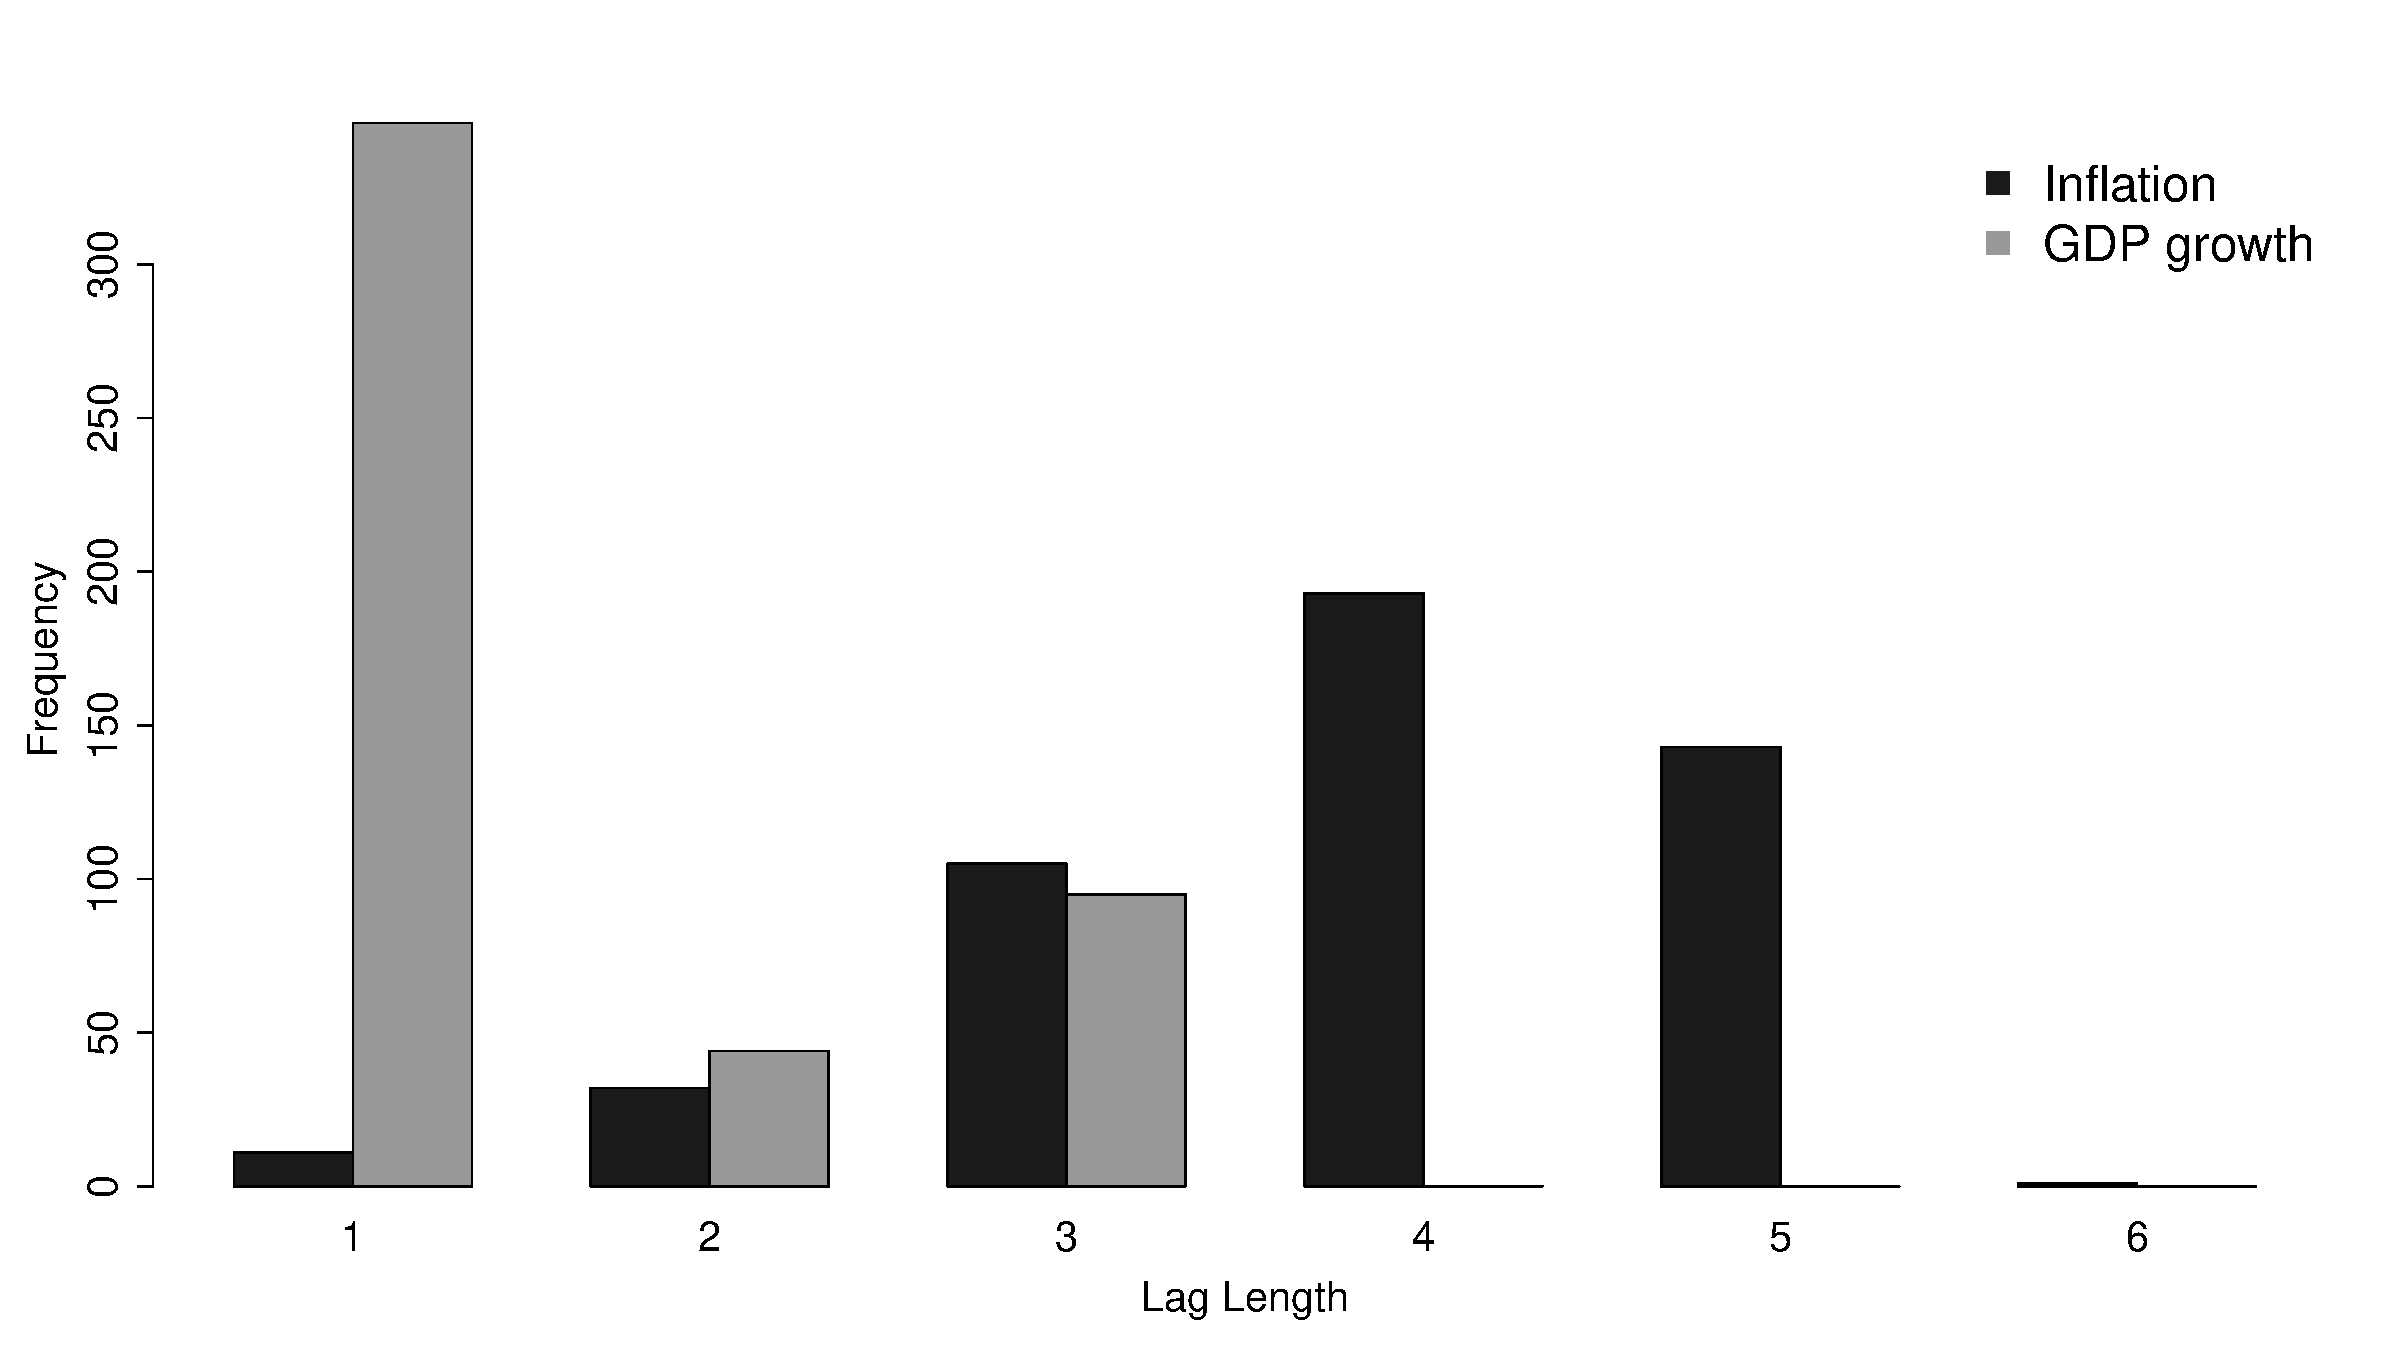
\includegraphics[width =\textwidth]{ar_lag_length_choice.pdf}
\caption{Empirical frequency of lag length choices $p \in \{1, 2, \ldots, 6\}$ in the AR($p$) model, separately for inflation and GDP growth. Frequencies are pooled across the G7 countries as well as all forecasting years and the spring and fall seasons. \label{fig:lag_length_choice}}
\end{figure}

\bibliographystyle{ecta}
\bibliography{references}

\end{document}
